\chapter{Dataset Descriptions}
\label{ch:data_description}

This chapter presents the datasets explored in this project, each representing different learning paradigms — classification (D-1, D-2) and clustering (D-3). Table~\ref{tab:dataset_summary} summarizes key dataset properties.

\begin{table}[H]
    \centering
    \caption{Summary of the datasets used in the project}
    \label{tab:dataset_summary}
    \begin{tabular}{|c|c|c|c|}
        \hline
        \textbf{Dataset} & \textbf{Learning Type} & \textbf{Samples} & \textbf{Features} \\
        \hline
        Raisin           & Classification        & 900              & 7                 \\
        HTRU2            & Classification        & 17,898           & 8                 \\
        Parking Birmingham & Clustering           & ~3,000 (cleaned) & 2-3               \\
        \hline
    \end{tabular}
\end{table}

\section{D-1: Raisin Dataset}
\label{sec:dataset_raisin}

The Raisin dataset, sourced from the UCI Machine Learning Repository \cite{raisin_dataset}, contains morphological features of two raisin types.
It contains morphological measurements of raisins, aiming to classify between \textit{Kecimen} and \textit{Besni} raisin types.

\begin{figure}[H]
    \centering
    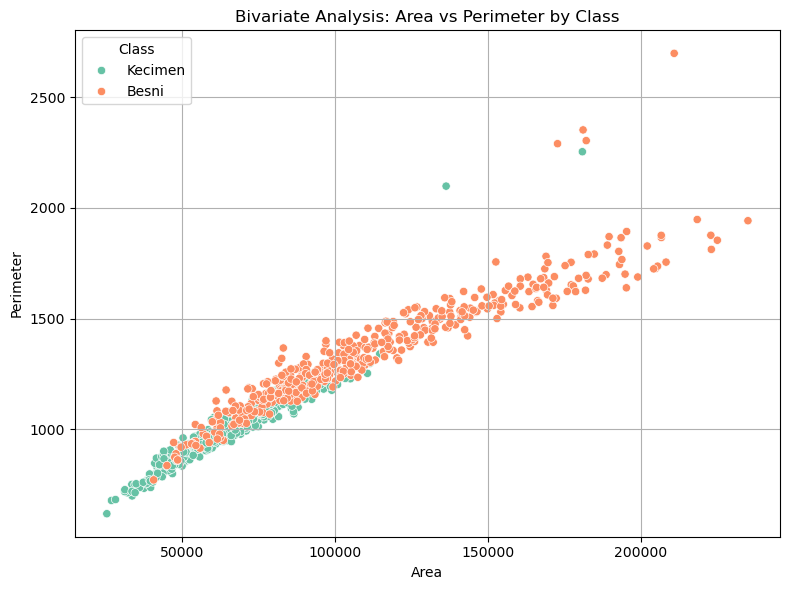
\includegraphics[width=0.6\textwidth]{figures/raisin_scatter.png}
    \caption{Bivariate plot of Area vs Perimeter by Raisin Class}
    \label{fig:raisin_scatter}
\end{figure}

Figure~\ref{fig:raisin_scatter} shows a clear distinction between classes, validating its suitability for binary classification tasks.

\section{D-2: HTRU2 Dataset}
\label{sec:dataset_htru2}

The HTRU2 dataset \cite{htru2_dataset} was selected for its numeric richness and binary classification challenge. HTRU2 (High Time Resolution Universe) data supports binary classification of pulsars vs non-pulsars. The dataset's numeric nature is ideal for probabilistic and distance-based models.

\begin{figure}[H]
    \centering
    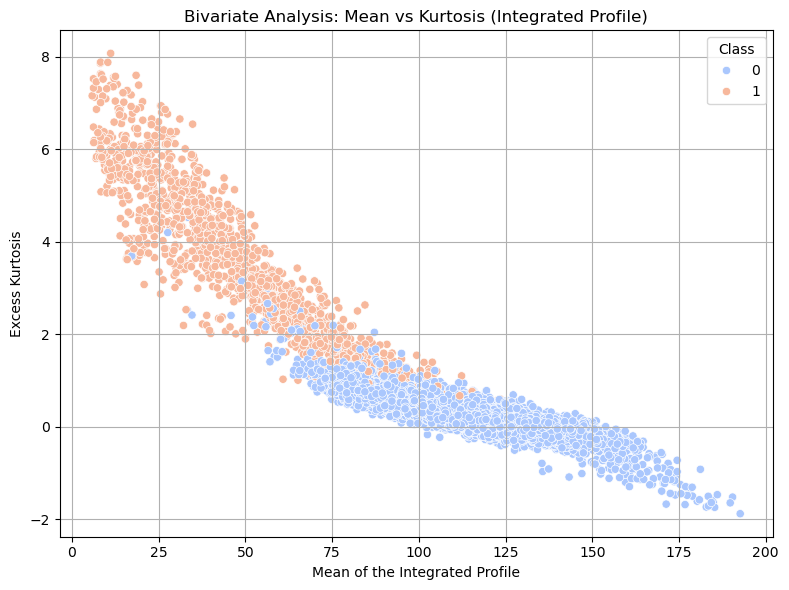
\includegraphics[width=0.6\textwidth]{figures/htru2_scatter.png}
    \caption{Bivariate plot of Mean vs Kurtosis (Integrated Profile)}
    \label{fig:htru2_scatter}
\end{figure}

As seen in Figure~\ref{fig:htru2_scatter}, separability exists between classes in selected feature pairs.

\section{D-3: Parking Birmingham Dataset}
\label{sec:dataset_parking}

Live parking data was obtained from Birmingham’s public data portal \cite{parking_dataset} and preprocessed for clustering. This dataset represents urban parking lot behavior, suited for unsupervised learning. It was preprocessed to retain occupancy and capacity features, which were scaled and clustered using K-Means.

\begin{figure}[H]
    \centering
    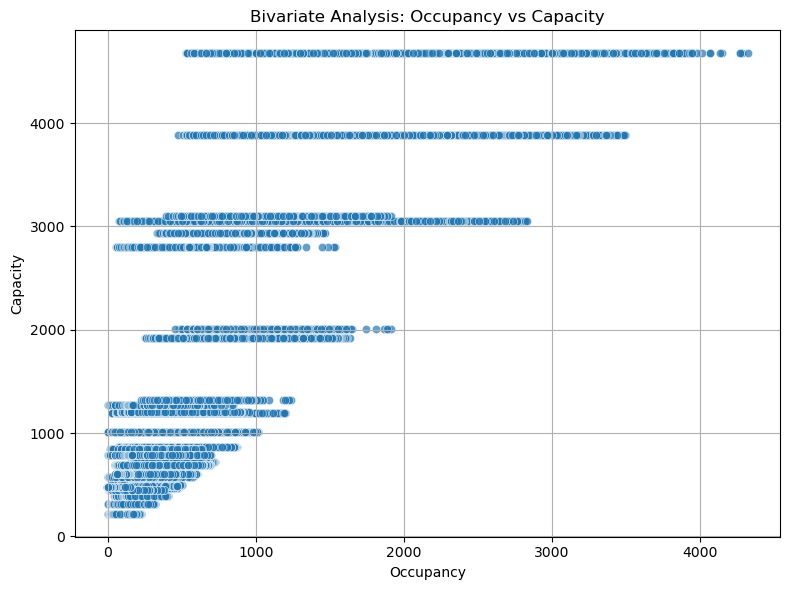
\includegraphics[width=0.6\textwidth]{figures/parking_scatter.png}
    \caption{Occupancy vs Capacity Bivariate Plot (Pre-clustering)}
    \label{fig:parking_scatter}
\end{figure}

Figure~\ref{fig:parking_scatter} highlights the spread of parking data before clustering, setting the stage for K-Means segmentation.

\section{Summary}
\label{sec:dataset_summary}

Table~\ref{tab:dataset_summary} summarizes dataset details. From classification of biological data (Raisins), and astrophysical signal interpretation (HTRU2), to smart city parking analytics, this project draws on diverse real-world data scenarios to showcase fundamental machine learning techniques.
